% Some of the discussion can be put inside the introduction part, depending on the content

% Include everything we have tried, what parameter we have turned.

% Very natural

% Introduction of the database and so on
\section{Context, Motivation and Goals}

Haussmanian renovations of Paris took place between 1853 and 1870. Commissioned by Emperor Napoleon III and directed by Georges Eugène Haussmann, the renovation significantly reshaped Paris. Crowded and gloomy medieval streets were demolished. Wide avenues, new parks, and squares were built. This transformation makes Paris a special example in the study of urbanization \cite{wiki_haussmanns}.

More than 1500 maps carefully describe Paris in the 18th and 19th centuries, and we can now easily digitize the maps and analysis the urbanization development in Paris on a computer. 

With all these data, the first problem to work on is precisely deriving what Paris looked like in different years. Maps always have errors, no matter how carefully they are drawn. We may have several maps of Paris published in the same year, but there are always some differences between them. 

In order to obtain a ground truth map of Paris for each year, one method is to align and take the average of all maps published that year. There are already applications where alignment can be performed manually by matching the corresponding points of two maps. However, this can be time-consuming if we have a large data set for analysis. This report discusses two alignment algorithms that would automate the process.

\section{Data set}

The data set contains 340 maps of Paris from the Bibliothèque Nationale de France (French national library, BnF). Each map is labeled by its publishing year, longitude and latitude converge. The earliest map in the data set is published in 1760, and the latest is in 1949. The histogram of the map publishing year is shown below in Figure \ref{his}.

\begin{figure}[h!]
\centering
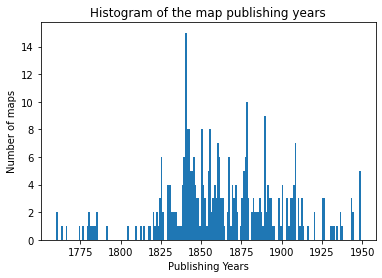
\includegraphics[scale=0.6]{Histogram.png}
\caption{Histogram of the map publishing years}
\label{his}
\end{figure}
% notebooks/Program/Phase%202%20KNN/Overlapping_knn.ipynb

\section{Prior work}

\subsection{Vectorization algorithm}

% We used a kernal ...
% Left: original map
% Right: Vectorized map
Vectorization of the map can be performed by one CNN-based algorithm \cite{remi_petitpierre}. The algorithm output the coordinates of the starting and ending point of all the road segment detected. We draw the vectorized map on a canvas of $10000 \times 10000$ pixels. The vectorized map is a 2D matrix. Each entry corresponds to one pixel in the map. The road pixels have a value of 1, and other pixels have a value of 0. Two examples of the vectorized map and its original map are shown below in Figure \ref{compare1} and \ref{compare2}. To better visualize the result, the road pixel is scaled to a value of 255. A dilation is applied with the kernel 
$K = \bigg(\begin{smallmatrix}
  1 & 1 & 1 & 1\\
  1 & 1 & 1 & 1\\
  1 & 1 & 1 & 1\\
  1 & 1 & 1 & 1\\
\end{smallmatrix}\bigg)$.

\begin{figure}[h!]
     \centering
     \begin{subfigure}{0.48\textwidth}
         \centering
         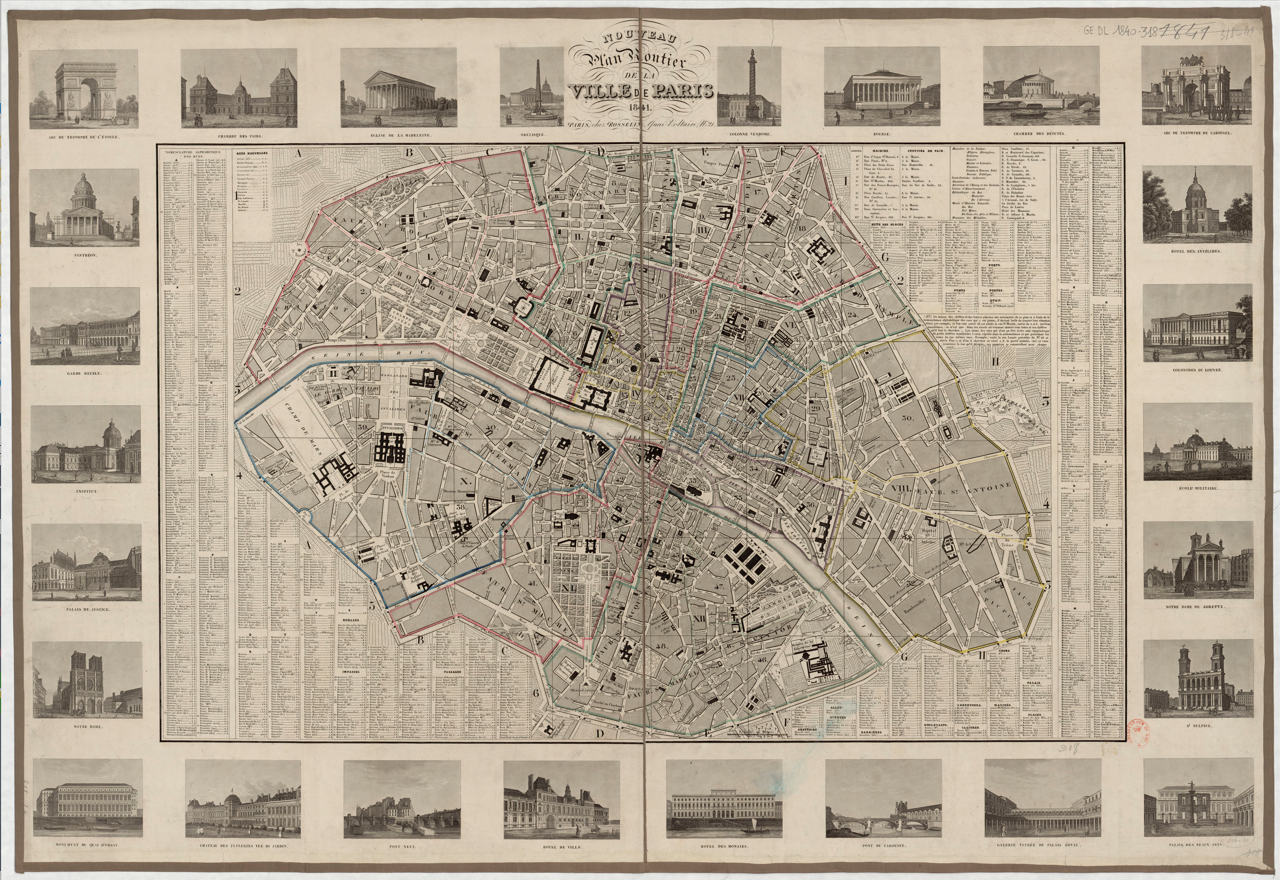
\includegraphics[width=\textwidth]{Images/mapA_native_screenshot.png}
         \caption{Original map}
         \label{compare::a}
     \end{subfigure}
     \hfill
     \begin{subfigure}{0.48\textwidth}
         \centering
         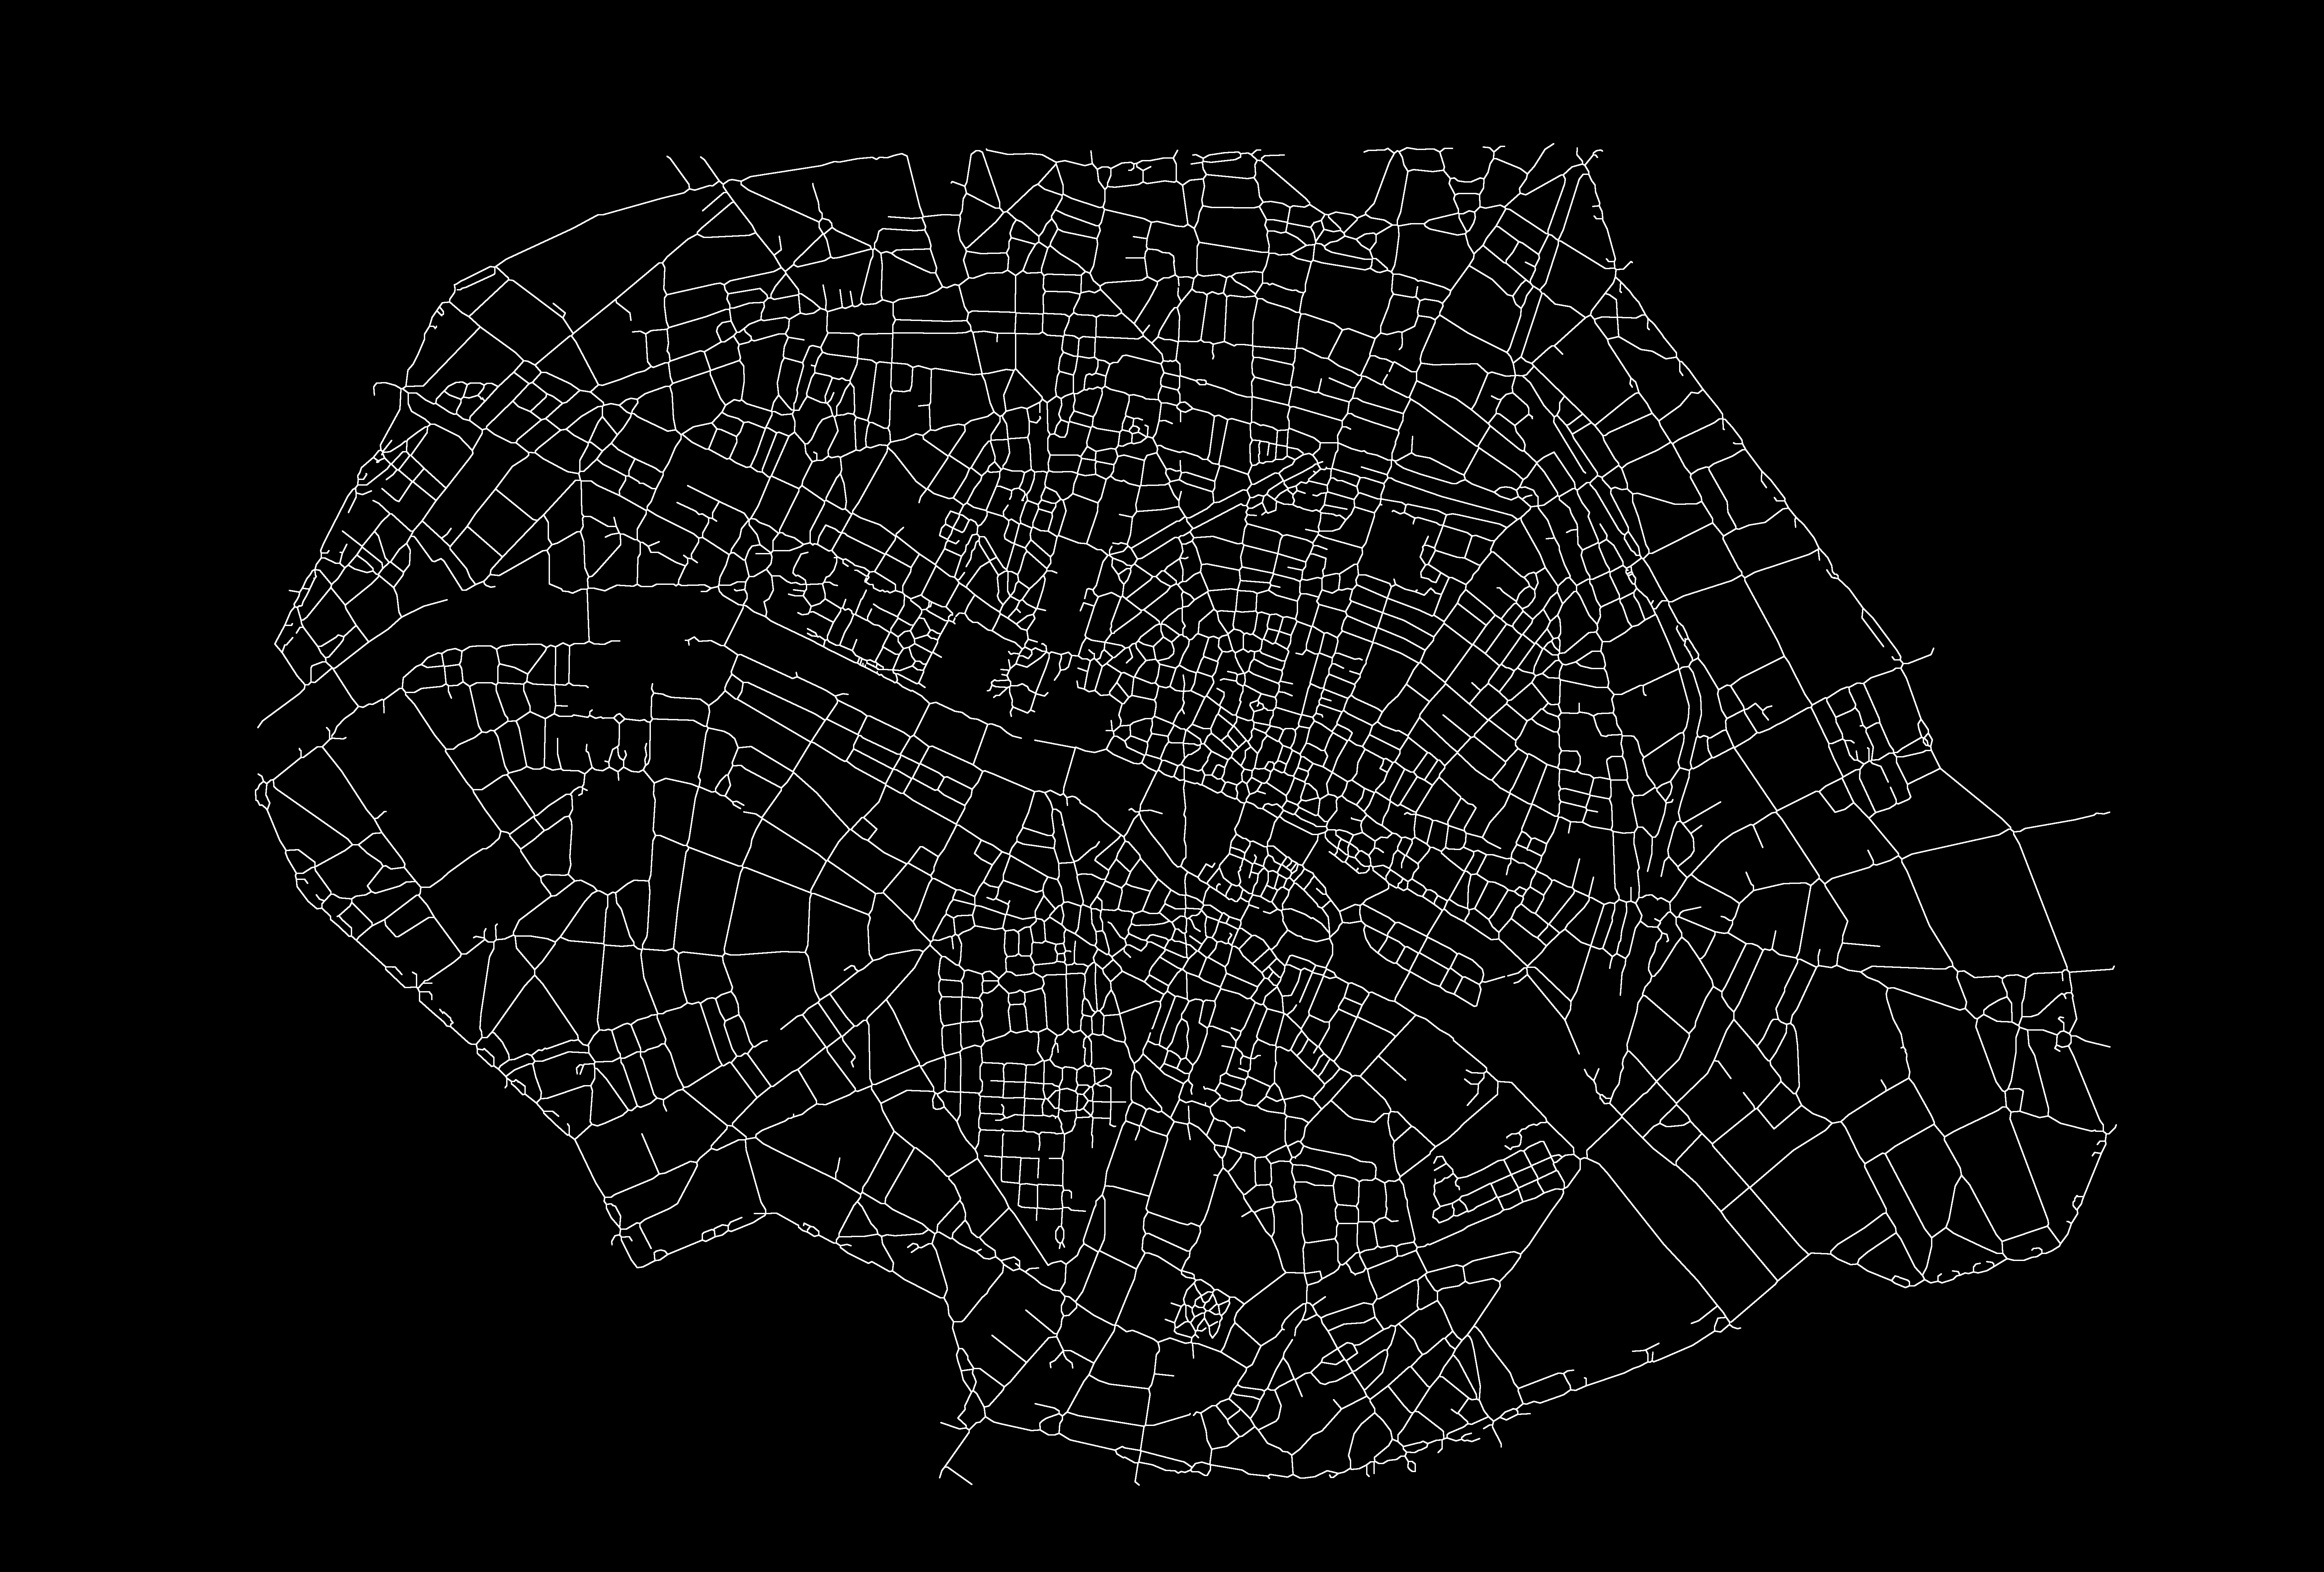
\includegraphics[width=\textwidth]{mapA_diated.png}
         \caption{Vectorized map}
         \label{compare::b}
     \end{subfigure}
        \caption{Original and vectorized version of the map \textit{Nouveau plan routier de la ville de Paris 1841}}
        \label{compare1}
\end{figure}

\begin{figure}[h!]
     \centering
     \begin{subfigure}{0.48\textwidth}
         \centering
         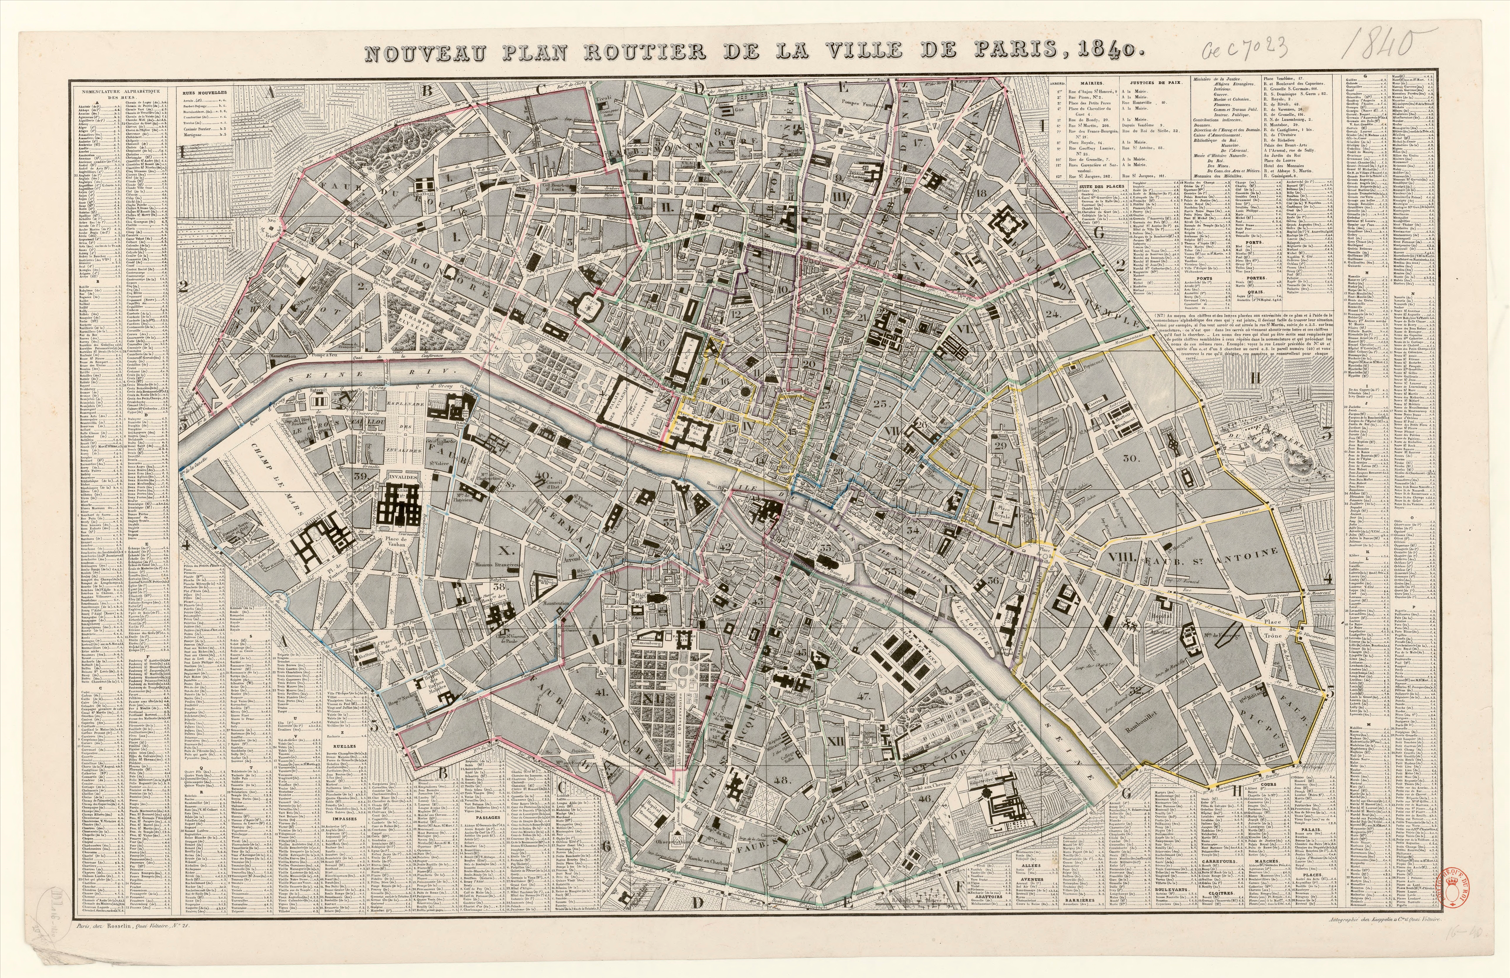
\includegraphics[width=\textwidth]{Images/mapB_native_screenshot.png}
         \caption{Original map}
         \label{compare::a}
     \end{subfigure}
     \hfill
     \begin{subfigure}{0.48\textwidth}
         \centering
         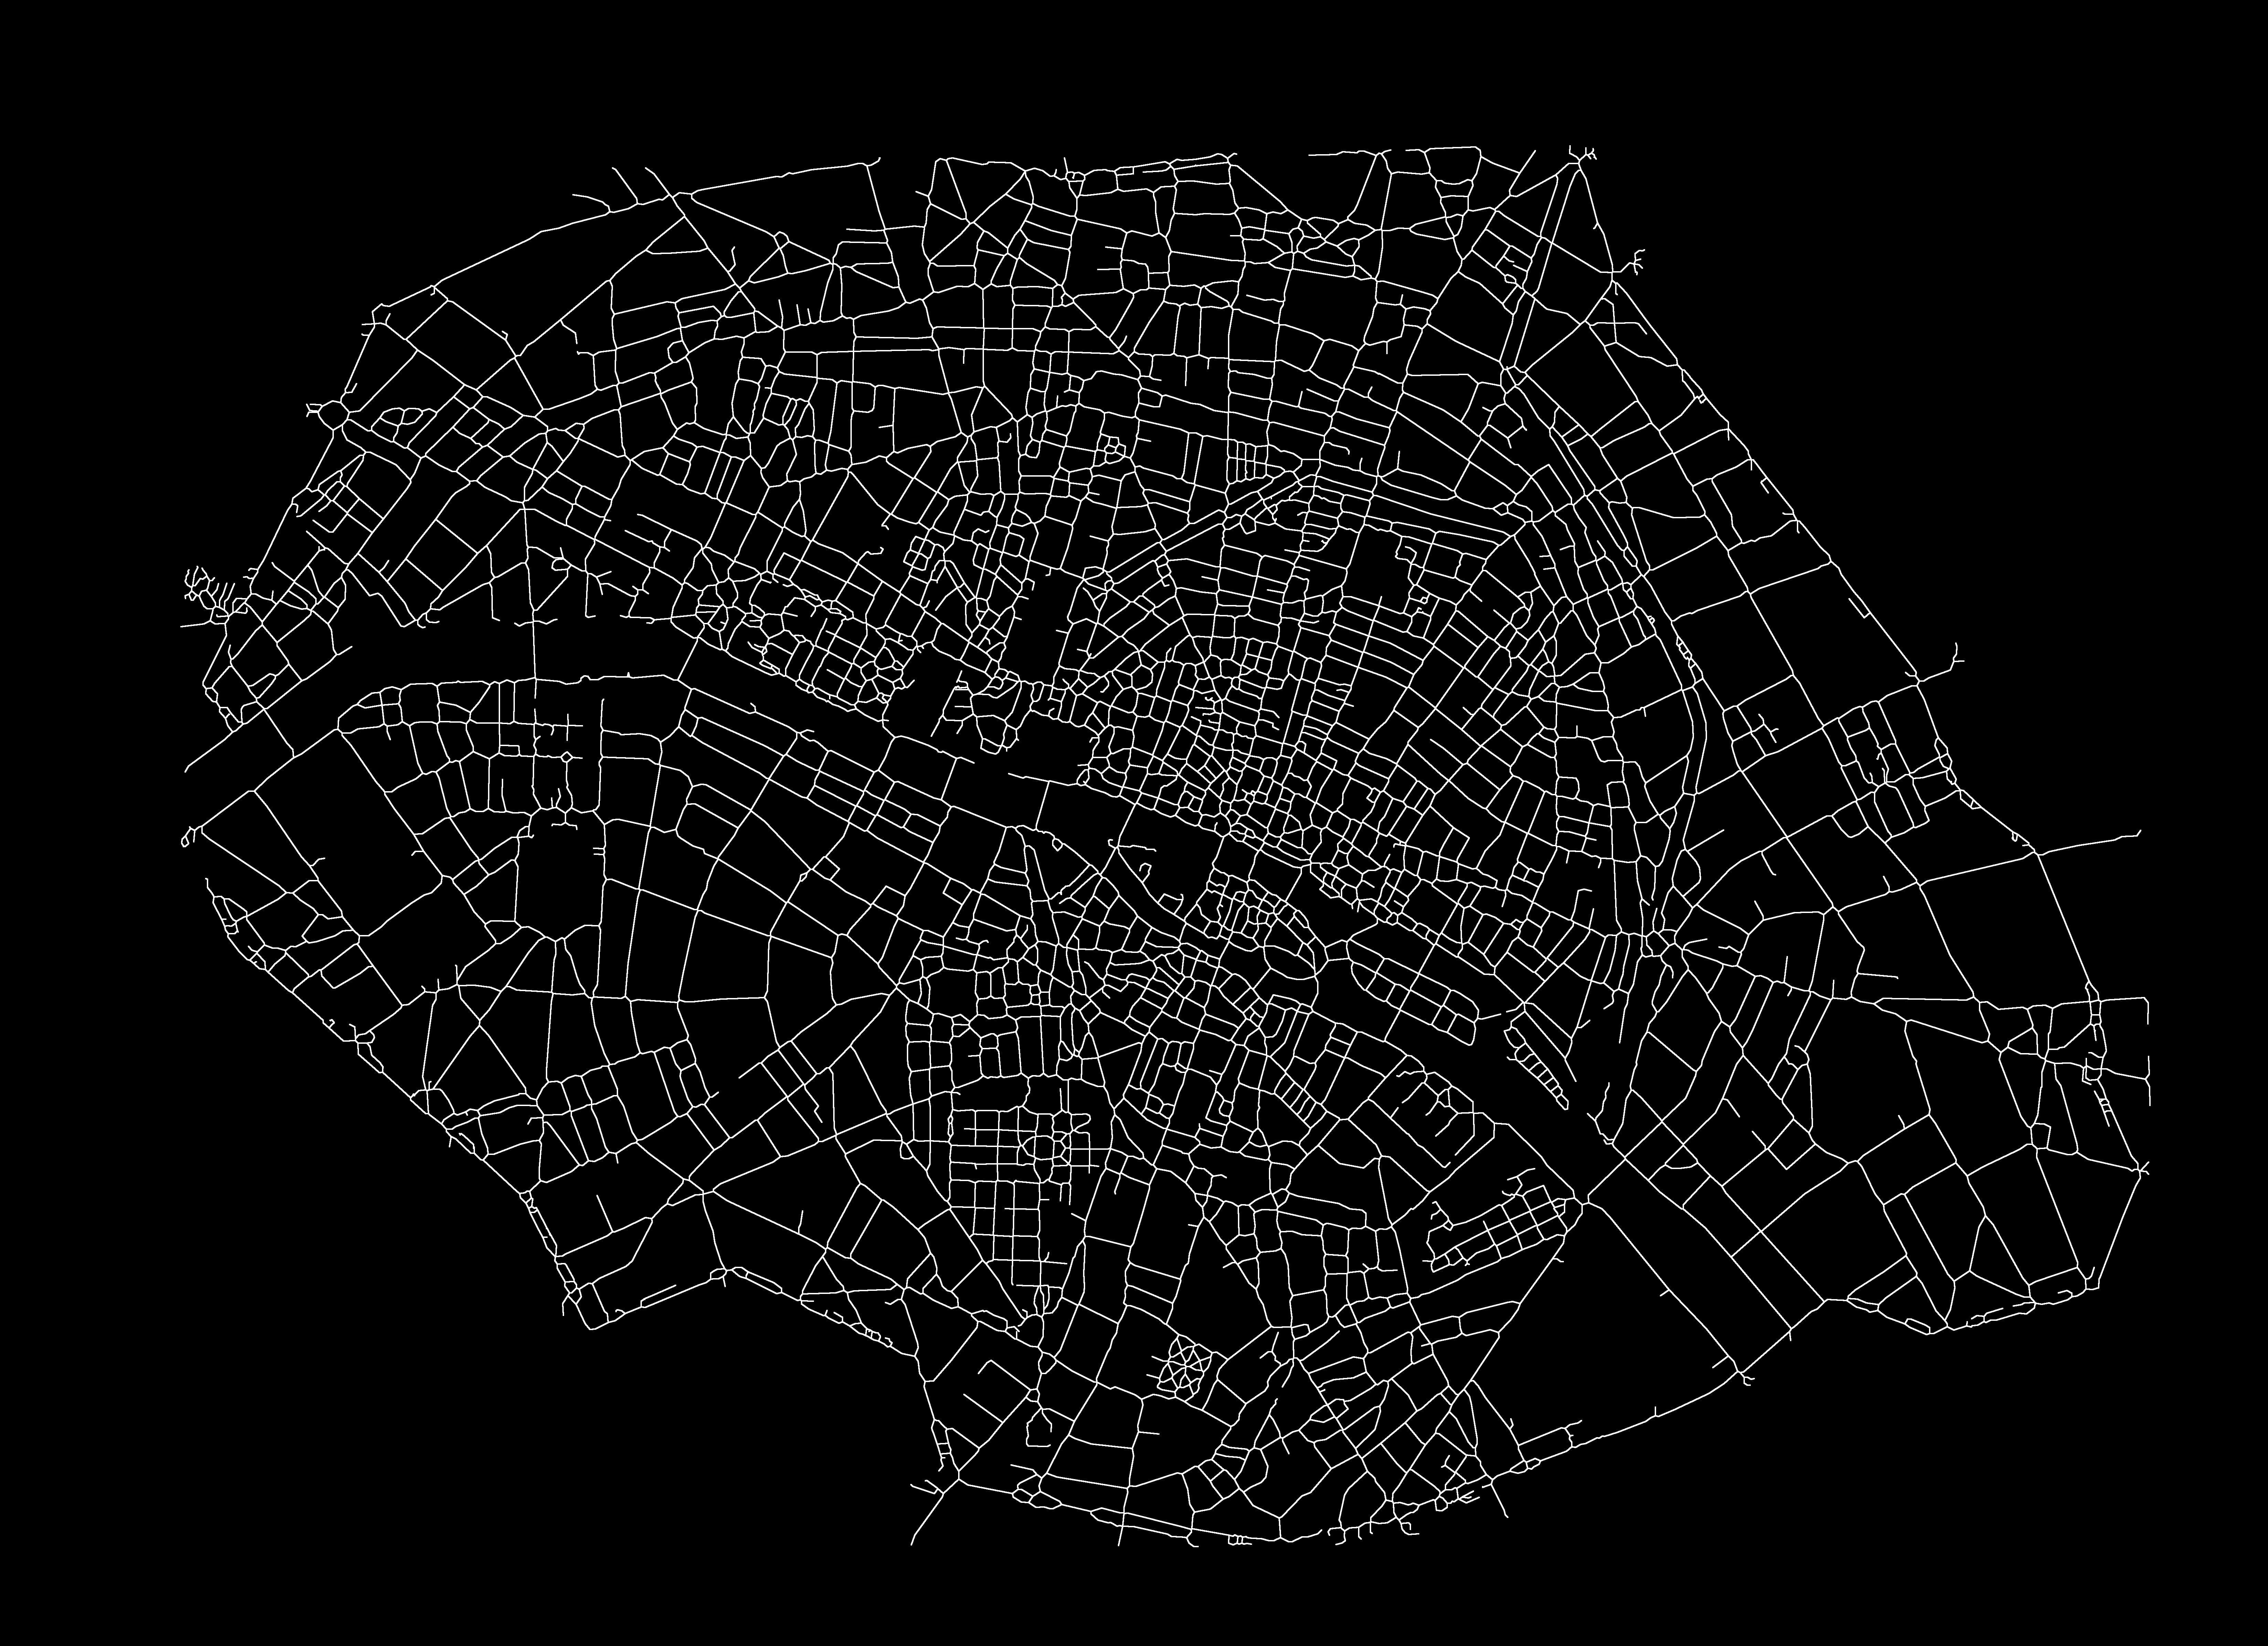
\includegraphics[width=\textwidth]{mapB_diated.png}
         \caption{Vectorized map}
         \label{compare::b}
     \end{subfigure}
        \caption{Original and vectorized version of the map \textit{Nouveau plan routier de la ville de Paris 1840}}
        \label{compare2}
\end{figure}
%notebooks/Phase%202%20KNN/Overlapping_knn.ipynb


% Describe why the naive one would not work, show some of the result by directly overlapping the maps together, and by using the transformation
\subsection{Alignment algorithm without ORB \cite{opencv_library}} 
One algorithm initially developed for image alignment \cite{mallick_2015_image} can be used to align the vectorized map we have. The algorithm tries to align the image with affine transformation, which combines rotation, translation(shift), scale, and shear. The affine transformation has six independent parameters. The algorithm used Enhanced Correlation Coefficient (ECC) Maximization \cite{mallick_2015_image} to find these parameters and align the maps.

\subsubsection{Method}
% Describe how we processed the map
% Overlapping_align_2_present.ipynb
The algorithm is a direct application of the tutorial given in [1], with \texttt{\footnotesize number\_of\_iterations} initialized as 5000 and \texttt{\small termination\_eps} initialized as $10^{-10}$ \cite{mallick_2015_image}.

Before feeding to the algorithm, the road pixel of the vectorized map is scaled to 255. A dilation is then applied with the kernel
$K = \bigg(\begin{smallmatrix}
  1 & 1 & 1 & 1\\
  1 & 1 & 1 & 1\\
  1 & 1 & 1 & 1\\
  1 & 1 & 1 & 1\\
\end{smallmatrix}\bigg)$,
followed by a Gaussian blur with \texttt{\small ksize} \cite{opencv_library} set to be $[5, 5]$

\subsubsection{Result} \label{ecc_result}

Map \textit{Nouveau plan routier de la ville de Paris 1841} and \textit{Nouveau plan routier de la ville de Paris 1840} are selected as alignment examples.

If two maps are directly overlapped, the result is shown in Figure \ref{geo}.

\begin{figure}[h!]
\centering
\includegraphics[width=0.9\textwidth]{Images/overlap1.png}
\caption{Direct overlap result of two map examples}
\label{geo}
\end{figure}

In comparison, the alignment result of the ECC Maximization algorithm discussed before is shown in Figure \ref{ecc}. 

\begin{figure}[h!]
\centering
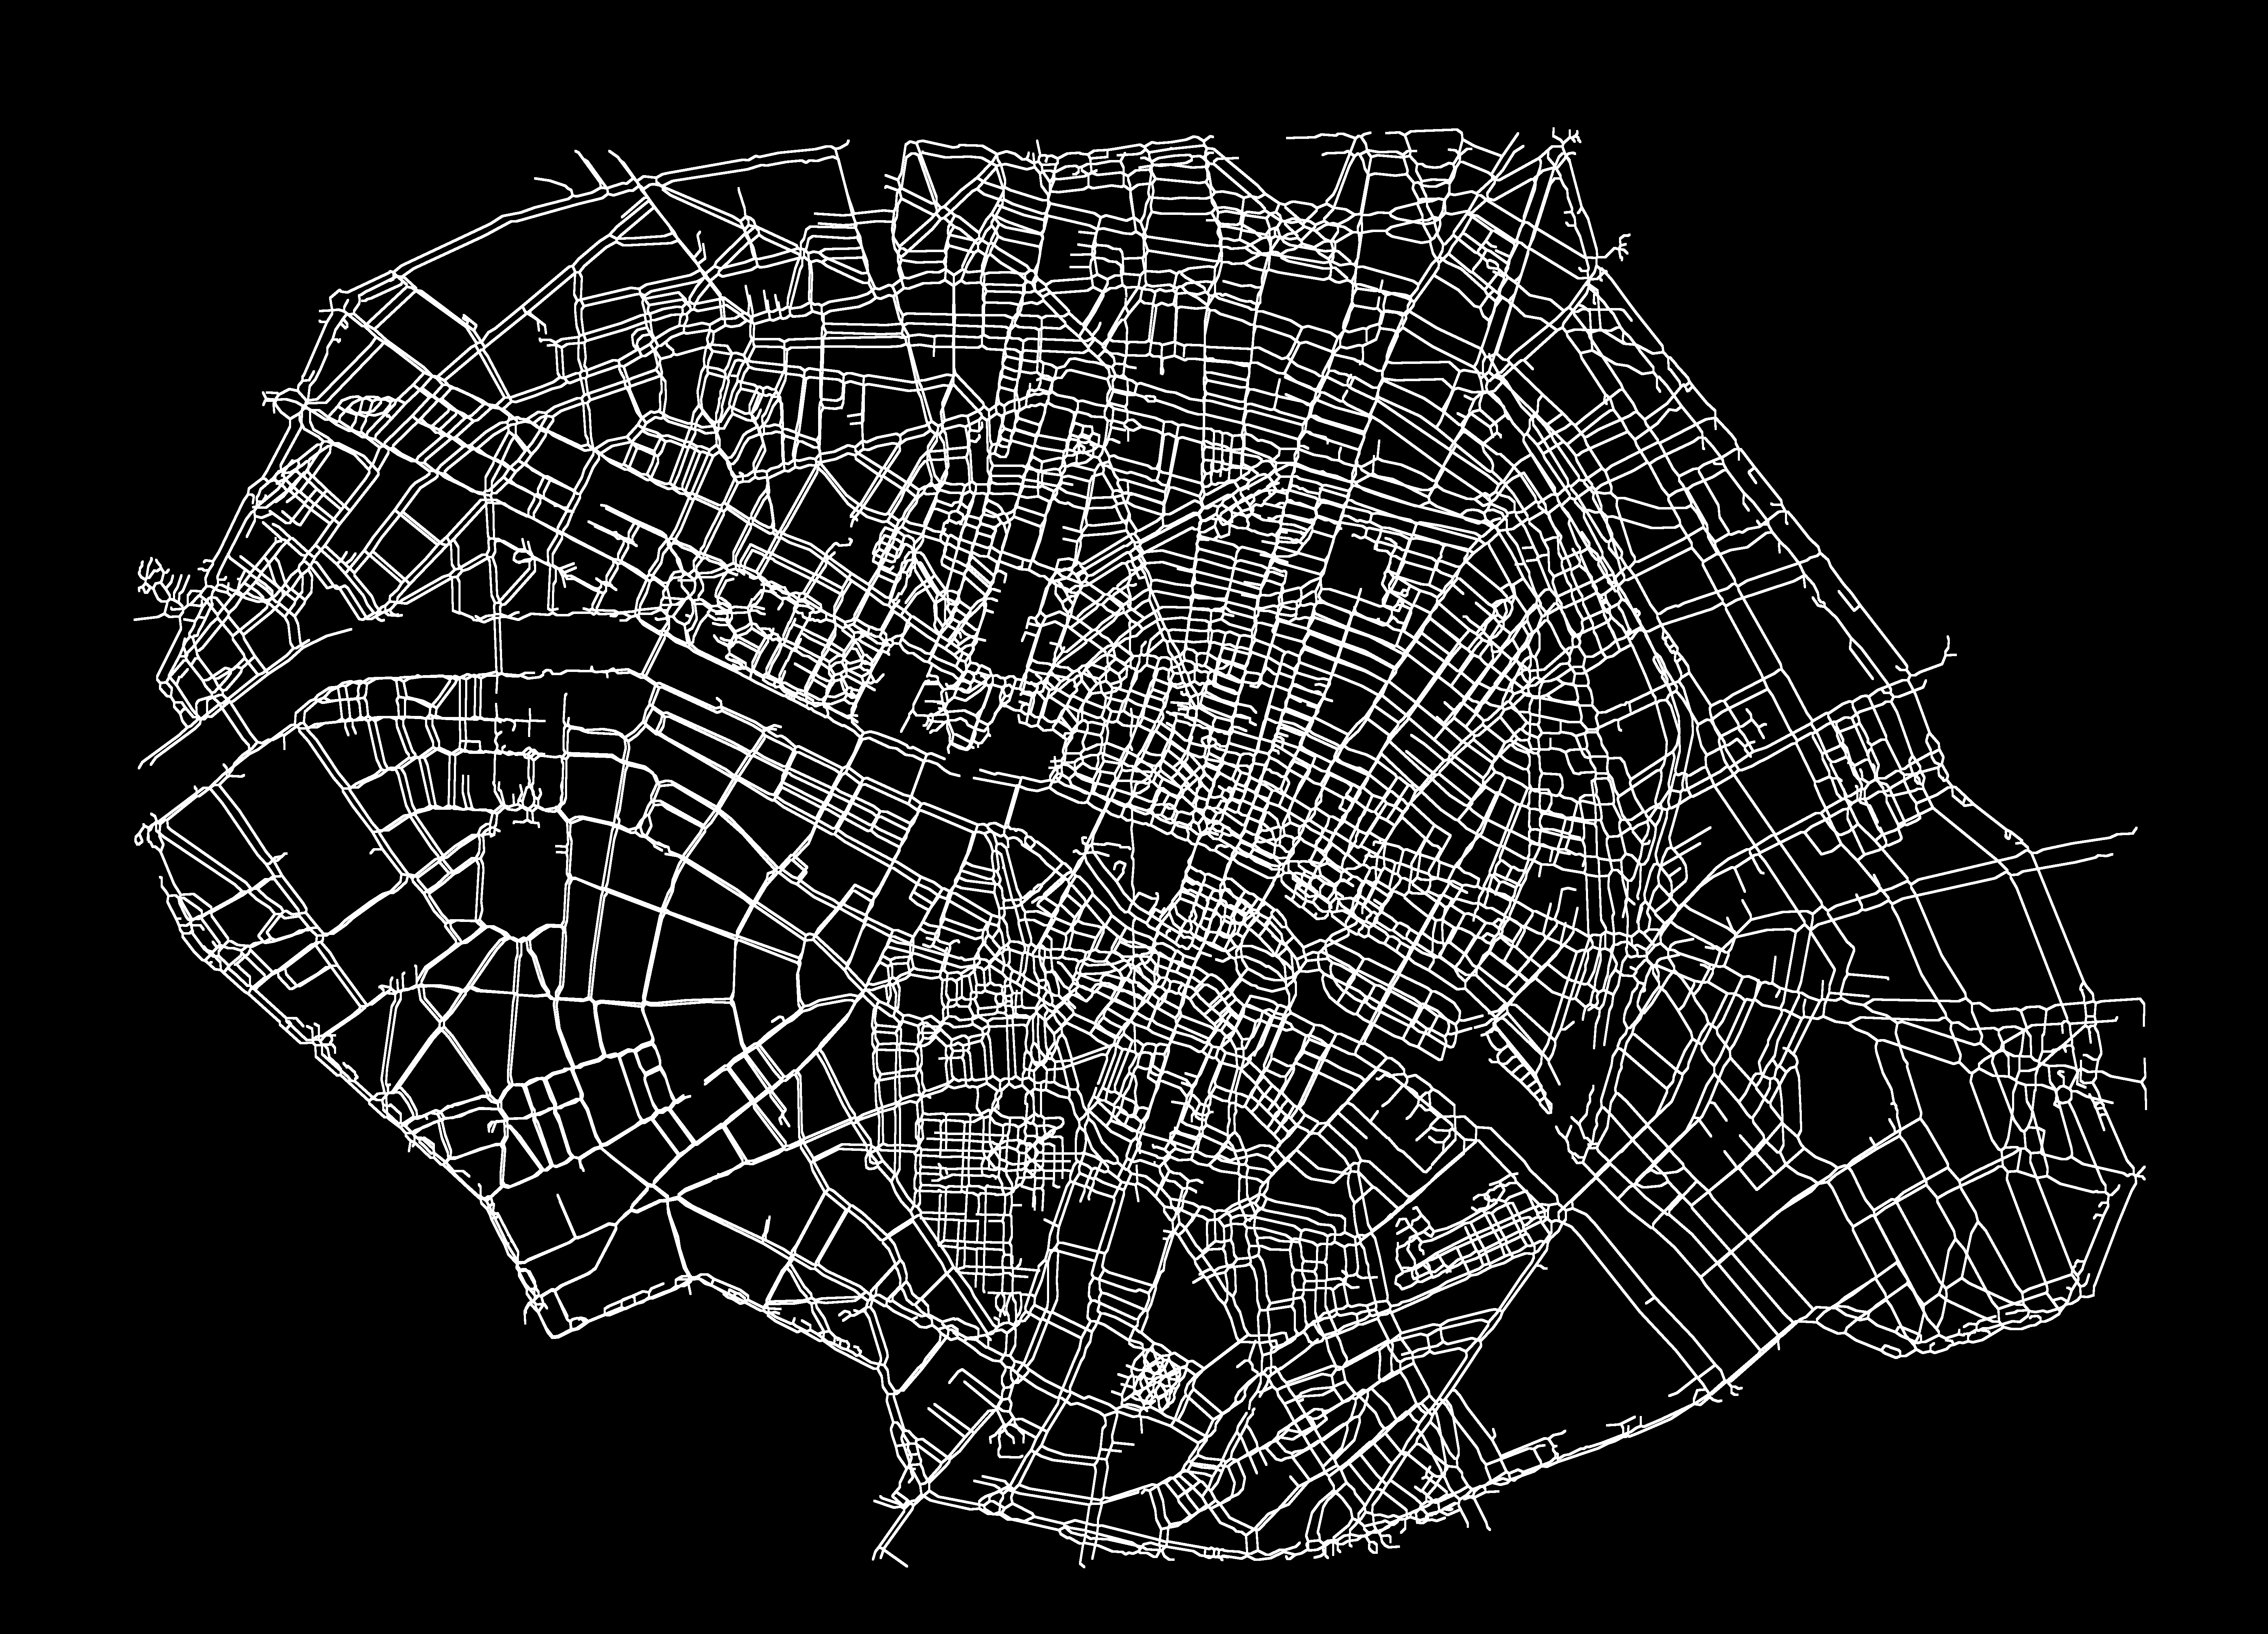
\includegraphics[width=0.9\textwidth]{Images/ECC_old.png}
\caption{Alignment result of the ECC maximization algorithm}
\label{ecc}
\end{figure}

\subsubsection{Discussion}
We chose these two maps as they have similar shapes but can not be aligned by directly overlapping with each other. In this case, the alignment algorithm's performance is more apparent.

Compare Figure \ref{geo} with Figure \ref{ecc}, ECC Maximization algorithm improve the alignment result. Generally, it can not do worse than simple overlapping. However, an affine transformation is too simple to align maps perfectly. In Figure \ref{ecc}, even though the bottom left corner is perfectly aligned, there are still misalignments in the upper right corner of two maps.